%%
%% This is file `sample-acmtog.tex',
%% generated with the docstrip utility.
%%
%% The original source files were:
%%
%% samples.dtx  (with options: `acmtog')
%% 
%% IMPORTANT NOTICE:
%% 
%% For the copyright see the source file.
%% 
%% Any modified versions of this file must be renamed
%% with new filenames distinct from sample-acmtog.tex.
%% 
%% For distribution of the original source see the terms
%% for copying and modification in the file samples.dtx.
%% 
%% This generated file may be distributed as long as the
%% original source files, as listed above, are part of the
%% same distribution. (The sources need not necessarily be
%% in the same archive or directory.)
%%
%% The first command in your LaTeX source must be the \documentclass command.
\documentclass[manuscript,review,anonymous]{acmart}

%% NOTE that a single column version is required for 
%% submission and peer review. This can be done by changing
%% the \doucmentclass[...]{acmart} in this template to 
%% \documentclass[manuscript,screen]{acmart}
%% 
%% To ensure 100% compatibility, please check the white list of
%% approved LaTeX packages to be used with the Master Article Template at
%% https://www.acm.org/publications/taps/whitelist-of-latex-packages 
%% before creating your document. The white list page provides 
%% information on how to submit additional LaTeX packages for 
%% review and adoption.
%% Fonts used in the template cannot be substituted; margin 
%% adjustments are not allowed.

\usepackage{amsmath} 
\usepackage{subfig}
\usepackage{booktabs}
\usepackage{multirow}
\usepackage[ruled,vlined]{algorithm2e}
\usepackage{bbm}
\usepackage[export]{adjustbox}

%%
%% \BibTeX command to typeset BibTeX logo in the docs
\AtBeginDocument{%
  \providecommand\BibTeX{{%
    \normalfont B\kern-0.5em{\scshape i\kern-0.25em b}\kern-0.8em\TeX}}}

%% Rights management information.  This information is sent to you
%% when you complete the rights form.  These commands have SAMPLE
%% values in them; it is your responsibility as an author to replace
%% the commands and values with those provided to you when you
%% complete the rights form.
\setcopyright{acmcopyright}
\copyrightyear{2021}
\acmYear{2021}
\acmDOI{10.1145/1122445.1122456}

%%
%% These commands are for a JOURNAL article.
%\acmJournal{TOG}
%\acmVolume{37}
%\acmNumber{4}
%\acmArticle{111}
%\acmMonth{8}

%%
%% Submission ID.
%% Use this when submitting an article to a sponsored event. You'll
%% receive a unique submission ID from the organizers
%% of the event, and this ID should be used as the parameter to this command.
%%\acmSubmissionID{123-A56-BU3}

%%
%% The majority of ACM publications use numbered citations and
%% references.  The command \citestyle{authoryear} switches to the
%% "author year" style.
%%
%% If you are preparing content for an event
%% sponsored by ACM SIGGRAPH, you must use the "author year" style of
%% citations and references.
\citestyle{acmauthoryear}

\newcommand{\el}[1]{
        \textcolor{magenta}{EL: #1}}

\newcommand{\dk}[1]{
        \textcolor{blue}{DK: #1}}
        
\newcommand{\pmu}[1]{
        \textcolor{orange}{PM: #1}}
        
\newcommand{\Rho}{\mathrm{P}}

\DeclareMathOperator*{\argmin}{arg\,min}
\DeclareMathOperator*{\argmax}{arg\,max}
%%
%% end of the preamble, start of the body of the document source.
\begin{document}

%%
%% The "title" command has an optional parameter,
%% allowing the author to define a "short title" to be used in page headers.
%\title{\dk{Sharing is Caring: Neighborhood Reuse for Privacy-Aware Collaborative Filtering Recommender Systems}}
\title{\emph{ReuseKNN}: Neighborhood Reuse for Privacy-Aware Collaborative Filtering}

%Controlling for Data Diffusion in Collaborative Filtering Recommender Systems
%%
%% The "author" command and its associated commands are used to define
%% the authors and their affiliations.
%% Of note is the shared affiliation of the first two authors, and the
%% "authornote" and "authornotemark" commands
%% used to denote shared contribution to the research.
%\author{Anonymous}
\author{Peter Müllner}
\email{pmuellner@know-center.at}
\affiliation{%
  \institution{Know-Center Gmbh}
  \city{Graz}
  \country{Austria}
}

\author{Dominik Kowald}
\email{dkowald@know-center.at}
\affiliation{%
  \institution{Know-Center Gmbh}
  \city{Graz}
  \country{Austria}
}

\author{Elisabeth Lex}
\affiliation{%
  \institution{Graz University of Technology}
  \city{Graz}
  \country{Austria}}
\email{elisabeth.lex@tugraz.at}

%%
%% By default, the full list of authors will be used in the page
%% headers. Often, this list is too long, and will overlap
%% other information printed in the page headers. This command allows
%% the author to define a more concise list
%% of authors' names for this purpose.
%\renewcommand{\shortauthors}{Trovato and Tobin, et al.}

%%
%% The abstract is a short summary of the work to be presented in the
%% article.
\begin{abstract}
In user-based \emph{KNN} recommender systems, recommendations are calculated based on the $k$ nearest neighbors of a target user.
That can pose a privacy risk as the target user could infer its neighbors' rating data.
In this work, we propose modifications to the inner workings 
%architecture 
of user-based \emph{KNN} to minimize the number of users who can infer other users' rating data. 
To that end, we present \emph{ReuseKNN}, a novel privacy-aware recommender system that preserves privacy through neighborhood reuse.
\emph{ReuseKNN} estimates a user's reusability as the degree to which the target user could reuse this user’s data for recommendations it may query in the future.
\emph{ReuseKNN} then scores users by a weighted average between similarity and reusability, and the highest scored users are used as neighbors for a target user. 
This trade-off between similarity and reusability serves as a proxy for users’ trade-off between accuracy and privacy.
In this paper at hand, we present the concept of neighborhood reuse and outline its potential to increasing privacy in user-based \emph{KNN} recommender systems.
Furthermore, we propose unpersonalized and personalized neighborhood reuse methods to estimate users' reusability and generate reusable neighborhoods in \emph{ReuseKNN}.
Additionally, our experiments on four different datasets from various domains, i.e., \emph{MovieLens 100k}, \emph{MovieLens 1M}, \emph{Jester}, and \emph{Goodreads}, reveal that \emph{ReuseKNN} yields substantially better trade-offs between users' accuracy and privacy compared to traditional user-based \emph{KNN}.
In detail, we show that \emph{ReuseKNN} improves privacy of traditional user-based \emph{KNN} recommender systems, at no or only marginal cost of accuracy. We hope that our results inspire future work to make traditional recommendation algorithms more privacy-aware by modifying their inner workings through neighborhood reuse.
\end{abstract}

%%
%% The code below is generated by the tool at http://dl.acm.org/ccs.cfm.
%% Please copy and paste the code instead of the example below.
%%

%%
%% Keywords. The author(s) should pick words that accurately describe
%% the work being presented. Separate the keywords with commas.
\keywords{Recommender System; Collaborative Filtering; Privacy; User-based KNN; Inference Attacks}


%%
%% This command processes the author and affiliation and title
%% information and builds the first part of the formatted document.
\maketitle

\section{Introduction}
Recommender systems often rely on collaborative filtering to generate recommendations.
However, collaborative filtering can pose severe risks to users' privacy, since, for example in the case of user-based \emph{KNN}, recommendations are generated based on data that is collected from the $k$ nearest neighbors of a target user.
The threat to users' privacy lies in their contribution to the generation of other users' recommendations.
In this regard, research in~\cite{ramakrishnan2001being} and~\cite{calandrino2011you} illustrates that users are susceptible to multiple privacy threats, such as, e.g., the inference of their private rating data. 
To alleviate this issue, several works proposed to use \emph{Differential Privacy}~\cite{dwork2014algorithmic} to protect users' data in user-based \emph{KNN} recommender systems~\cite{zhu2014effective,lu2015security}.
As an alternative to \emph{Differential Privacy}, recent research~\cite{badsha2017privacy,zhang2021privacy} utilized \emph{Homomorphic Encryption}~\cite{gentry2009fully} in user-based \emph{KNN} recommender systems to encrypt users' data and provide stronger privacy guarantees. 
In contrast to the works above, which aim to ensure privacy by modifying users' data, in our work, we aim to increase the privacy of users by proposing modifications to the inner workings 
%architecture 
of user-based \emph{KNN} recommendation methods that do not modify the users' data. 
In particular, we present our novel \emph{ReuseKNN} recommender system, which minimizes the number of users that could infer other users' rating data.
For example, consider our schematic illustration on the left hand side in Figure~\ref{fig:approach}.
Here, we compare a traditional user-based \emph{KNN} recommender system, i.e., \emph{UserKNN}, to \emph{ReuseKNN}.
Instead of utilizing \emph{Bob}'s, \emph{Tim}'s, and \emph{John}'s rating data for generating recommendations for \emph{Alice} as traditional \emph{UserKNN} would do, \emph{ReuseKNN} reuses \emph{Bob} in all recommendations and thus, \emph{Tim} and \emph{John} do not contribute to the generation of \emph{Alice}'s recommendations.
This means that \emph{Alice} cannot infer \emph{Tim}'s and \emph{John}'s rating data and as such, their privacy is protected.
In detail, before selecting a user as neighbor, \emph{ReuseKNN} estimates the user's reusability, which is the degree to which the target user could reuse this user's data for multiple recommendations. 
To quantify a user's reusability, \emph{ReuseKNN} utilizes both unpersonalized and personalized neighborhood reuse methods.
In contrast to traditional \emph{UserKNN}, which selects neighbors based on their similarity to the target user, \emph{ReuseKNN} scores users by a weighted average between similarity and reusability.
Then, \emph{ReuseKNN} chooses the $k$ highest scored users to be neighbors for a target user. 
This trade-off between similarity and reusability serves as proxy for users' trade-off between accuracy and privacy.

To illustrate the impact of reusing neighbors in user-based \emph{KNN} recommender systems on users' accuracy-privacy trade-off, we compare \emph{ReuseKNN} with traditional \emph{UserKNN} on four different datasets, i.e., \emph{MovieLens 100k}, \emph{MovieLens 1M}, \emph{Jester}, and \emph{Goodreads}. 
We find that \emph{ReuseKNN} yields a better accuracy-privacy trade-off than \emph{UserKNN}, i.e., it increases users' privacy at no or only marginal cost of accuracy.
Especially \emph{ReuseKNN} utilizing the personalized neighborhood reuse method shows the best results over all four datasets.
Our experiments also indicate that \emph{ReuseKNN} substantially limits the growth of a user's neighborhood to a minimum, in contrast to traditional \emph{UserKNN}.
Additionally, we demonstrate that \emph{ReuseKNN} does not utilize the same neighborhood for all target users and as such, does not show a bias towards a small set of neighbors.
Instead, it tends to assign users their own distinct set of reusable neighbors.

Taken together, the three main contributions of our paper are as follows: 
First, we discuss the concept of reusing neighbors for privacy-aware collaborative filtering and its impact on users' privacy.
Second, we outline our novel \emph{ReuseKNN} recommender system and propose multiple unpersonalized and personalized neighborhood reuse methods that estimate to what degree a target user could reuse its neighbors.
Third, we conduct extensive experiments on four datasets with different characteristics from multiple domains and present how \emph{ReuseKNN} improves users' accuracy-privacy trade-offs in user-based collaborative filtering. 

Other research works focused on protecting users' privacy through modifying their data.
In contrast, we propose modifications to the inner workings 
%architecture 
of user-based \emph{KNN} to decrease the number of users that could infer other users' rating data and as such, we increase privacy of these users.
To the best of our knowledge, we are the first utilizing reusable neighborhoods to improve users' accuracy-privacy trade-offs in user-based \emph{KNN} recommender systems.
We hope that our findings motivate other researchers to also modify the inner workings of traditional recommender systems to make them more privacy-aware.

%With that we desire to give an example of how simple adaptions to the inner workings of traditional recommendation algorithms could alleviate their users' privacy issues.

%%%%%%%%%%%%%%%%%%%%%%%%%%%%%%%%%%%%%%%%%%%%%%%%%%%%%%%%%%%%%%%%%%
\section{Approach}
\begin{figure*}[!t]
    \centering
    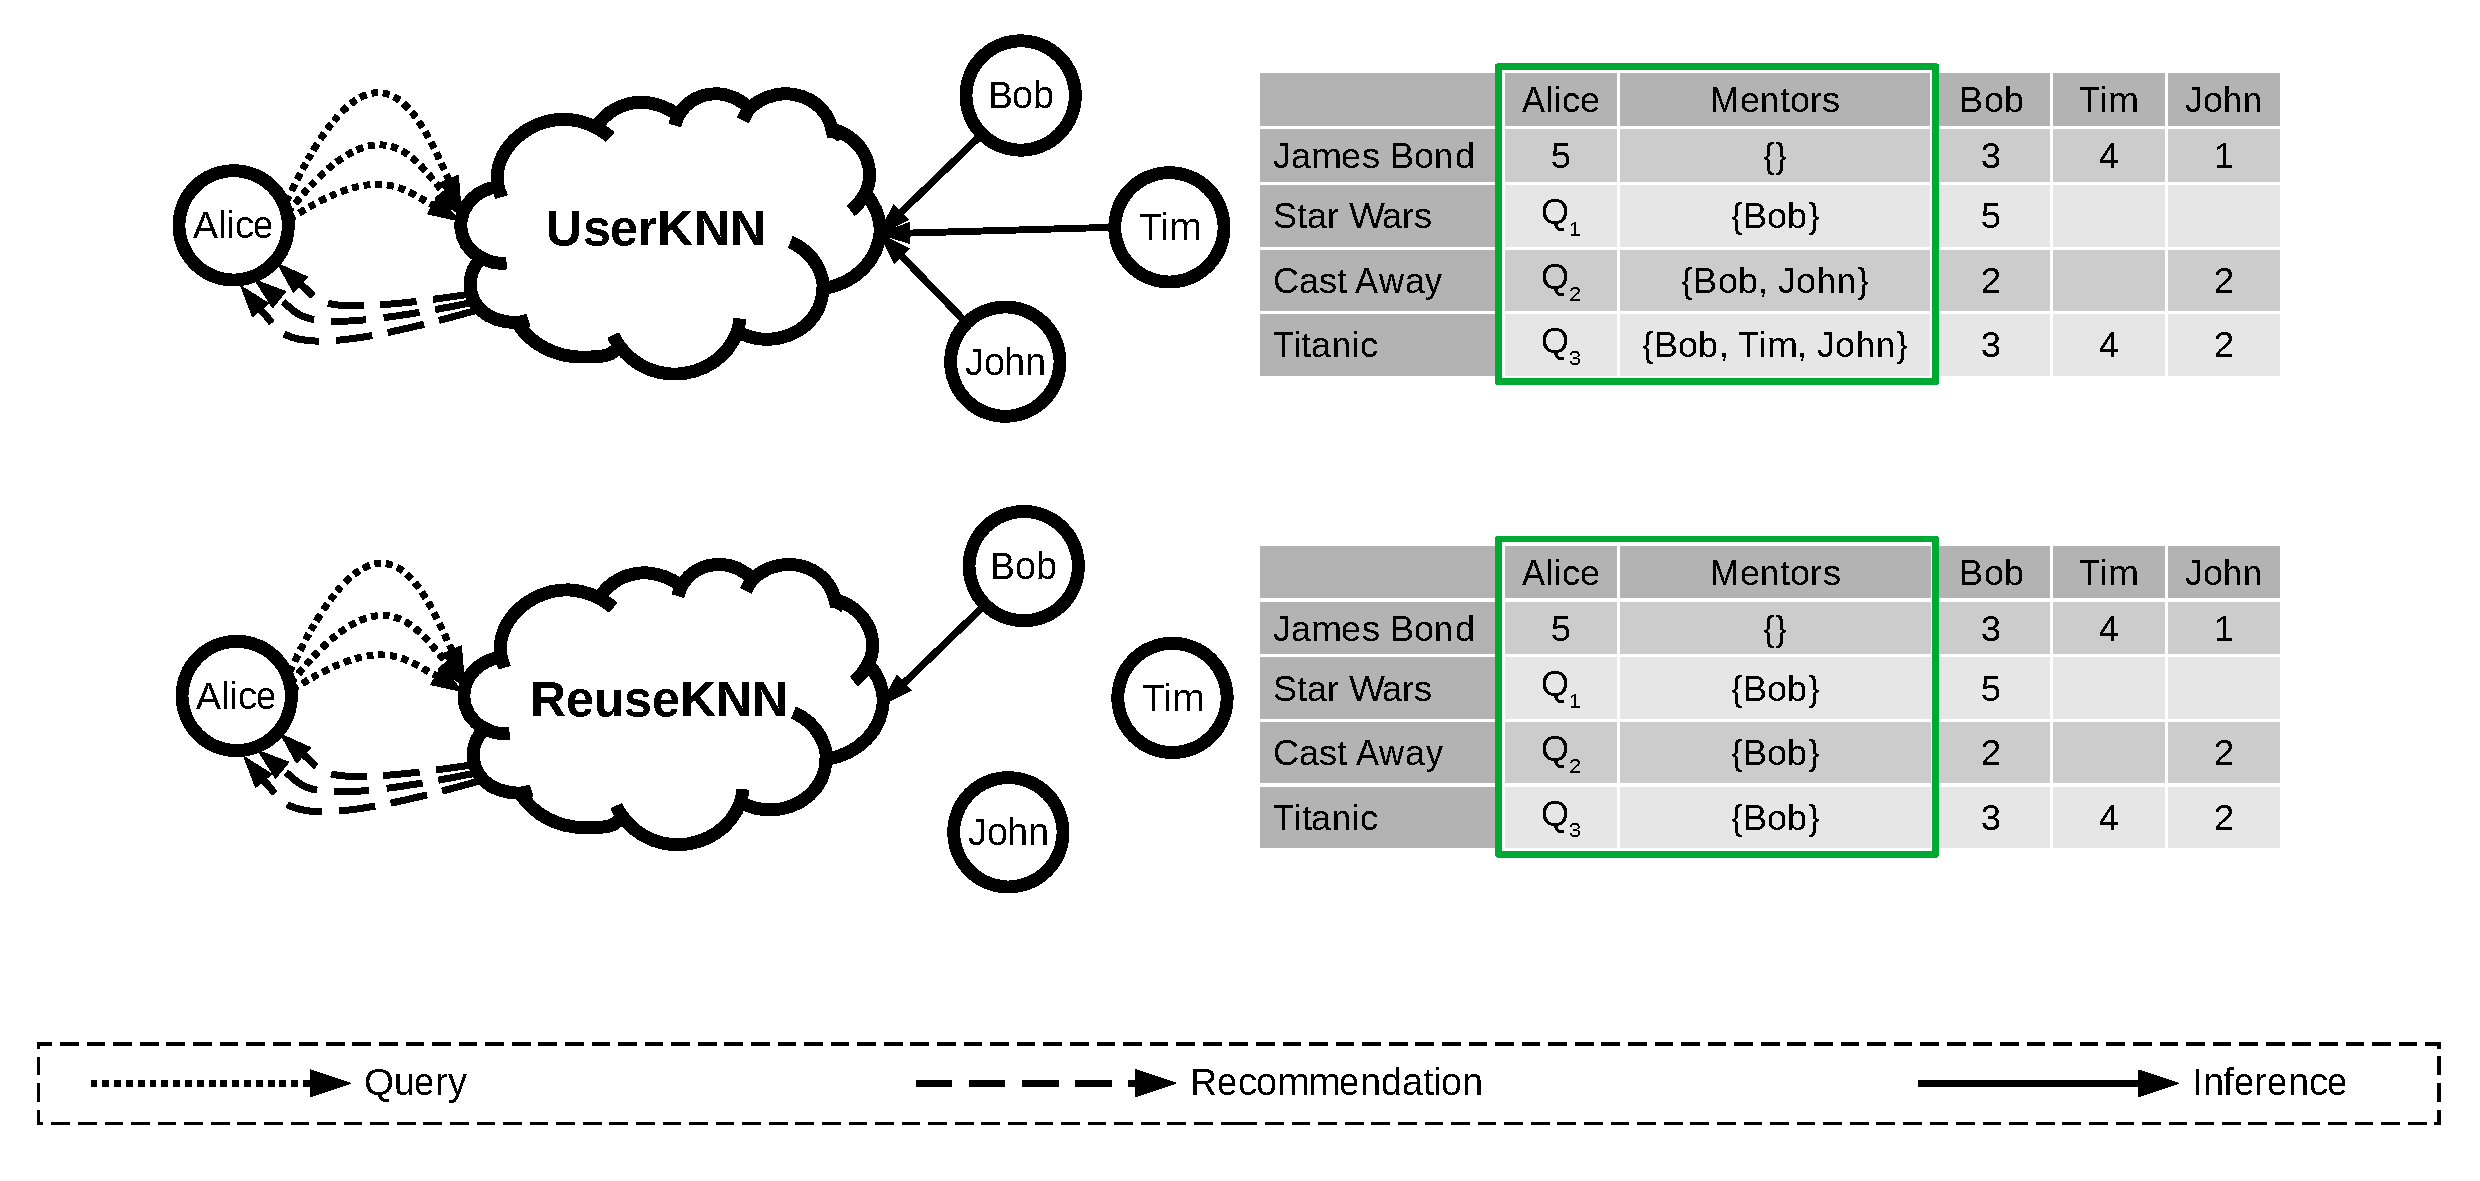
\includegraphics[width=\textwidth]{figures/approach.pdf}
    \caption{
    (Left) Schematic illustration of our novel \emph{ReuseKNN} recommender system compared to traditional \emph{UserKNN}. 
    In \emph{ReuseKNN}, \emph{Bob} is reused for all of \emph{Alice}'s recommendation queries.
    Thus, \emph{Alice} cannot infer \emph{Tim}'s and \emph{Bob}'s rating data.
    (Right) Rating data of all users plus \emph{Alice}'s three recommendation queries, $Q_1$, $Q_2$, and $Q_3$ and her neighbors $N_{Alice}$ across these three queries. 
    %In \emph{UserKNN}, \emph{Alice}'s recommendations are based on the rating data of her neighbors \emph{Bob}, \emph{Tim}, and \emph{John}.
    In detail, the threat to users' privacy is that each of \emph{Alice}'s neighbors rated at least one item she has rated, i.e., \emph{James Bond}. Plus, upon recommendation of \emph{Cast Away}, she knows that some of her neighbors also rated \emph{Cast Away}. By gradually adding specific ratings and querying recommendations, \emph{Alice} could successively reveal parts of \emph{Tim}'s and \emph{John}'s rating data.
    With \emph{ReuseKNN}, \emph{Bob} is reused for all three recommendation queries. Obviously, this means that \emph{Tim}'s and \emph{John}'s data is protected against inference.
    }
    \label{fig:approach}
\end{figure*}

User-based \emph{KNN} recommender systems generate an estimated rating score for a recommendation query $Q_{u, i}$ of \emph{target user} $u$ and \emph{target item} $i$ by utilizing the ratings of other users that have rated $i$.
In detail, for every item $i$, for which target user $u$ queries an estimated rating score, i.e., $i \in Q_u$, the recommender system $\mathcal{R}$ select $k$ users that rated $i$, i.e., the nearest neighbors $N^k_{u, i}$ for $u$ and $i$.
Then, $\mathcal{R}$ estimates $u$'s rating score for $i$, by considering the ratings of $N^k_{u, i}$, i.e., the recommendation $\mathcal{R}^k(u, i)$.
Thus, the $k$ nearest neighbors $N^k_{u, i}$ contribute to target user $u$'s estimated ratings and, this way, also to $u$'s recommendations.
Across multiple recommendation queries $Q_u$ of target user $u$, we define the set of $u$'s neighbors as $N_u = \bigcup_{i \in Q_u} N^k_{u, i}$.

Based on these definitions, in traditional user-based \emph{KNN} recommender systems, the recommender system's response $\mathcal{R}^k(u, i)$ to the target user's recommendation query $Q_{u, i}$ depends on the $k$ nearest neighbors $N^k_{u, i}$.
For a succeeding item $j$, the recommendation $\mathcal{R}^k(u, j)$ depends on another set of $k$ nearest neighbors $N^k_{u, j}$.
In Figure~\ref{fig:approach}, we illustrate the generation of multiple recommendations for target user \emph{Alice} with a traditional user-based \emph{KNN} recommender system, i.e., \emph{UserKNN}. 
We see that after recommending \emph{Star Wars}, \emph{Cast Away}, and \emph{Titanic}, target user \emph{Alice}'s set of neighbors $N_{Alice}$ comprises \emph{Bob}, \emph{Tim}, and \emph{John}.
\emph{Bob} contributes to three recommendations, \emph{John} to two recommendations and \emph{Tim} to one recommendation. 
Consider \emph{Alice} adding a rating for \emph{Titanic} to her existing rating for \emph{James Bond}.
If the recommender system yields the recommendation \emph{Cast Away}, \emph{Alice} knows that there exists at least one user that rated \emph{Titanic}, \emph{James Bond}, and \emph{Cast Away}.
However, since only one user, i.e., \emph{John}, rated these items, \emph{Alice} revealed parts of \emph{John}'s rating data, i.e., \emph{John}'s rating for \emph{Cast Away}.
This by itself is a breach of \emph{John}'s privacy.
%Plus, even incomplete knowledge of John's rating data is a strong threat to Bob's privacy.
%For example, incomplete knowledge could boost the effectiveness of other kinds of attacks, e.g., Sybil attacks~\cite{calandrino2011you}.
%Furthermore, John contributes to more of Alice's recommendations than Tim and thus, John has a higher susceptibility to inference attacks by Alice than Tim~\cite{ramakrishnan2001being}.
%However, technically, Alice could still infer not only the rating data of John, but also of all users that contributed to her recommendations.
%More concretely, from a privacy perspective, a user could be both, an attacker by itself, but also exposed to others' inference attacks.
This means that despite target user $u$ being solely aware of $u$'s own rating data and the recommendations $u$ receives, $u$ could infer the rating data of its neighbors by applying probing techniques~\cite{calandrino2011you,ramakrishnan2001being}, which means that all neighbors of $u$ are exposed to $u$'s potential inference attacks.
Additionally, we highlight that in user-based \emph{KNN} recommender systems, a user typically (i) queries recommendations, and (ii) contributes to the recommendations of other users.
As such, a user could be an attacker to other users, but at the same time, be also exposed to others' inference attacks.

In our work, we propose \emph{ReuseKNN}, a novel user-based \emph{KNN} recommender system reducing the exposure of users to inference attacks by leveraging our family of neighborhood reuse methods.
In \emph{ReuseKNN}, we redirect the users' exposure by reusing a target user's neighbors to generate recommendations. 
Our intuition is that reusing a target user $u$'s neighbors leads to other users not having to serve as neighbors for $u$.
With that, we can decrease users' exposure and increase their privacy.
Before describing our neighborhood reuse approach in more detail, we give a more formal definition of \emph{UserKNN}.

\subsection{Traditional \emph{UserKNN} Recommender System}
\label{subsec:userknn}
As mentioned, a traditional user-based \emph{KNN} recommender system, i.e., \emph{UserKNN}, generates an estimation $\hat{r}_{u, i}$ of a target user $u$'s preference for item $i$ by leveraging the data of $u$'s $k$ nearest neighbors $N^k_{u, i}$ for item $i$ according to some similarity measurement $sim$. This is given by:
\begin{equation}\label{eq:knn}
    \hat{r}_{u, i} = \frac{\sum_{n \in N^k_{u, i}} sim(u, n) \cdot r_{n, i}}{\sum_{n \in N^k_{u, i}} sim(u, n)}
\end{equation}
where $r_{n, i}$ is the rating of neighbor $n$ for item $i$ and $sim$ denotes a similarity function which measures the conformity between target user $u$ and neighbor $n$.
Typically, Cosine similarity is used as a similarity function due to its efficiency and ability to provide accurate recommendations~\cite{bagchi2015performance,verma2020comparative}.

In our example illustrated in Figure~\ref{fig:approach}, target user \emph{Alice} has rated the movie \emph{James Bond} and is now querying movie recommendations from the \emph{UserKNN} recommender system.
For \emph{Alice}'s first query, i.e., \emph{Star Wars}, \emph{UserKNN} selects \emph{Bob} as neighbor for \emph{Alice}, since \emph{Bob} is the only user that rated both, \emph{James Bond} and \emph{Star Wars}.
For \emph{Alice}'s second recommendation query, i.e., \emph{Cast Away}, \emph{UserKNN} selects \emph{Bob} and \emph{John} to be neighbors of \emph{Alice}.
Thus, the set of \emph{Alice}'s neighbors across multiple recommendation queries, i.e., $N_{Alice}$, now comprises \emph{Bob} and \emph{John}.
Finally, in a query for \emph{Titanic}, \emph{UserKNN} selects \emph{Bob}, \emph{Tim}, and \emph{John} as neighbors for \emph{Alice}.
In total, \emph{UserKNN} has selected three users, i.e., \emph{Bob}, \emph{Tim}, and \emph{John} to be neighbors of target user \emph{Alice}.
Hence, there is the possibility that \emph{Alice} could infer the rating data of \emph{Bob}, \emph{Tim} and \emph{John}. 
We now describe how this is different in case of our novel \emph{ReuseKNN} approach.\footnote{To some extent, also traditional \emph{UserKNN} reuses a target user $u$'s neighbors, as it tends to not select completely disjoint sets of neighbors for each of $u$'s recommendations.
However, the selection of neighbors is solely based on similarity and thus, agnostic to whether neighbors could be reused. This is contrary to our proposed \emph{ReuseKNN} recommender system, which actively incorporates neighbors' reusability to increase privacy.}

% From a privacy perspective, a user could attain two roles: \emph{susceptible} and \emph{attacker}.
% If the recommender system selects user $n$ to serve as neighbor in at least one recommendation for target user $u$, $n$ is also a mentor of $u$.
% Due to $n$ being $u$'s mentor, $n$ attains the role of a susceptible.
% That means that $n$ is susceptible to $u$'s inference attacks.
% Clearly, $u$ then attains the role of an attacker.
% Also, we highlight that in typical $k$-nearest neighbor collaborative filtering recommender system, a user (i) queries recommendations and (ii) contributes in the recommendations for other users.
% As such, a user could be susceptible to inference, but still be an attacker to other users.

\subsection{Our Novel \emph{ReuseKNN} Recommender System}
\label{subsec:reuseknn}
In order to provide accurate recommendations for one user whilst ensuring privacy of others, the paper at hand proposes the \emph{ReuseKNN} recommender system, which utilizes a novel family of neighborhood reuse methods.
Instead of decreasing the number of neighbors per target user, i.e., $N_u$, by using fewer neighbors per recommendation query, i.e., $N_{u, i}$, \emph{ReuseKNN}'s primary goal is to decrease the number of neighbors per target user whilst not limiting the number of neighbors that contribute to the generation of a recommendation in order to keep accuracy high~\cite{herlocker1999algorithmic,herlocker2002empirical}.

In particular, the key feature of \emph{ReuseKNN} is to reuse a target user's previously utilized neighbors whenever feasible.
With that, it reduces the number of users that are added to the target user's set of neighbors across multiple recommendation queries.
As shown in Figure~\ref{fig:approach}, \emph{ReuseKNN} redirects queries for multiple neighbors, i.e., \emph{Tim} and \emph{John}, to \emph{Bob}.
Thus, all recommendations for \emph{Alice} are based solely on neighbor \emph{Bob}, whereas \emph{Tim} and \emph{John} are not neighbors and thus, are protected against inference attacks by \emph{Alice}.
More detailed, for \emph{Alice}'s first recommendation query, i.e., \emph{Star Wars}, \emph{ReuseKNN} works in the same way as traditional \emph{UserKNN} and thus, selects \emph{Bob} as neighbor.
However, for the second recommendation query, i.e., \emph{Cast Away}, \emph{ReuseKNN} differs from \emph{UserKNN}.
Instead of increasing \emph{Alice}'s set of neighbors $N_{Alice}$ by using both, \emph{Tim} and \emph{John} as neighbors for this recommendation, \emph{ReuseKNN} reuses neighbors from $N_{Alice}$.
In detail, since neighbor \emph{Bob} already rated \emph{Cast Away}, \emph{ReuseKNN} reuses \emph{Bob} for \emph{Alice}'s recommendation of \emph{Cast Away}.
Moreover, we note that the rating of \emph{John} is in line with the rating of \emph{Bob}.
As such, including \emph{John} as neighbor would have no valuable advantage over reusing \emph{Bob} on \emph{Alice}'s recommendation.
Similarly, in the third recommendation query, i.e., \emph{Titanic}, \emph{ReuseKNN} does not add any additional neighbors for \emph{Alice} since neighbor \emph{Bob} has also rated \emph{Titanic}.
Plus, utilizing also \emph{Tim} and \emph{John} would not have any substantial benefit since their average rating corresponds to \emph{Bob}'s rating.
Overall, instead of selecting three different users as neighbors as \emph{UserKNN} does, and thus exposing these users' data to \emph{Alice}, \emph{ReuseKNN} reuses \emph{Alice}'s neighbors in her recommendations and thereby, prohibits inference attacks by \emph{Alice} on the users outside her neighborhood.

\subsubsection{Formalizing Neighborhood Reuse} 
For $Q_u$ being $u$'s recommendation queries, i.e., the set of items for which target user $u$ queries estimated rating scores, and $N^k_{u, i}$ being the $k$ nearest neighbors of $u$ for item $i$ used in estimating the rating score of $i$, \emph{ReuseKNN} aims to identify the minimal set of neighbors across multiple recommendation queries such that it minimizes the cardinality of $N_u = \bigcup_{i \in Q_u} N^k_{u, i}$
whilst keeping high accuracy of $u$'s recommendations.
Our \emph{ReuseKNN} recommender system does not only consider the similarity $sim(u, n)$ between target user $u$ and neighbor $n$, but also the extent to which the recommender system could reuse $n$'s rating data across multiple of $u$'s future recommendation queries, i.e., $reusability(n|u)$, which depends on our neighborhood reuse methods presented in the remainder of this work.
For this trade-off between similarity and reusability, we do not directly utilize the similarity and reusability scores, since both scores represent different measurements.
Instead, we trade-off the ranks of the similarity and reusability scores.
This accuracy-privacy trade-off can be formalized as weighted average between similarity and reusability:
\begin{align}
    \label{eq:tradeoff}
    score(n|u) &= \lambda \cdot rank(sim(u, n)) + (1 - \lambda) \cdot rank(reusability(n|u)) \\
    N^k_{u, i} &=\ \stackrel{k}{\argmax_{n \in U_i}} score(n|u)
\end{align}
where $U_i$ are all users that rated $i$ and \emph{ReuseKNN} selects the highest scored $k$ users, i.e., $N^k_{u, i}$, to contribute to target user $u$'s recommendation for item $i$ and thus, are added to $u$'s set of neighbors $N_u$.
Furthermore, $\lambda \in [0; 1]$ is used to trade accuracy (i.e., $sim$) for privacy (i.e., $reusability$).
In the paper at hand, we set the trade-off parameter $\lambda=0.5$ to equally account for both, accuracy and privacy.
By focusing on reusing neighbors across multiple recommendation queries, \emph{ReuseKNN} keeps the set of $u$'s neighbors minimal, and thus, increases the number of users that are protected against inference attacks.

To measure $reusability$ of neighbors, \emph{ReuseKNN} relies on our family of implicit and explicit neighborhood reuse methods.
Implicit neighborhood reuse methods nudge the recommender system into selecting neighbors for a target user that are most likely also reusable for the target user's future recommendation queries.
Explicit neighborhood reuse methods go one step further and not only nudge the recommender system into selecting reusable neighbors, but also explicitly reuse as many neighbors as possible.
In the following, we detail our proposed implicit and explicit neighborhood reuse methods.

%%%%%%%%%%%%%%%%%%%%%%%%%%%%%%%%%%%%%%%%%%%
\subsubsection{Implicit Neighborhood Reuse}
\label{subsubsec:implicitreuse}
In this work, we propose to reuse neighbors of a target user across multiple recommendation queries, such that other users' exposure to inference attacks is alleviated, whilst preserving the accuracy of recommendations the target user receives.
Our implicit neighborhood reuse methods do not explicitly reuse neighbors, but create an artificial bias towards selecting those neighbors in all future recommendations.
Neighbors are selected not only based on similarity but based on a trade-off between similarity and reusability as outlined in Equation~\ref{eq:tradeoff}.
In the following paragraphs, we discuss two methods for increasing the reusability of neighbors selected by the recommender system: (i) the unpersonalized \emph{Popularity} approach, and (ii) the personalized \emph{Gain} approach.

\vspace{2mm} \noindent \emph{Unpersonalized Neighborhood Reuse: Popularity.}
Intuitively, the more popular an item, the more likely it is that a target user will query an estimated rating score for this item.
Our \emph{Popularity} method relies on this observation and thus, estimates for how many recommendation queries the recommender system could reuse a neighbor's data.
Thus, our \emph{Popularity} approach promotes neighbors if they rated a lot of popular items.
Also, it penalizes neighbors that either rated only a few items or a lot of unpopular items. 
In detail, the reusability score of neighbor $n \in N_{u, i}$ of target user $u$ and item $i$ is defined by:
\begin{equation}
    %reusability(n|u) = reusability(n) = \sum_{r_{n, i} \in R_n} \frac{|\{ v \in U: \exists r_{v, i} \in R_v \}|}{|U|} \label{eq:popularity}
    reusability(n|u) = reusability(n) = \sum_{i \in I_n} \frac{|U_i|}{|U|} \label{eq:popularity}
\end{equation}
%where $R_n$ is the set of ratings of user $n$ and $U$ is the set of all users.
where $I_n$ are the items $n$ rated, $U_i$ are the users that rated item $i$, and $U$ is the set of all users.
Thus, $reusability(n)$ is defined as the summed-up popularity scores of the items $n$ has rated and measures the expected number of a random user's recommendation queries to which $n$ could contribute to as a neighbor. 
This means that $reusability(n)$ according to our \emph{Popularity} approach measures the reusability of a neighbor with respect to the average user and thus, does not depend on target user $u$. 

\vspace{2mm} \noindent \emph{Personalized Neighborhood Reuse: Gain.}
When generating an estimated rating score for item $i$ and target user $u$, the recommender system utilizes a neighbor $n$'s rating for $i$.
In general, \emph{ReuseKNN} selects those neighbors for a target user, whose rating data could be reused across multiple of the target user's recommendation queries.
That means that $n$'s rated items $I_n$ should cover most of the target user $u$'s future recommendation queries, i.e., $Q_u$.
Obviously, \emph{ReuseKNN} does not know for which items target user $u$ will query ratings in the future. 
Instead of asking how much of a user's future ratings a neighbor could cover, our \emph{Gain} method asks how much of a target user's ratings a neighbor could have covered in the past, i.e., how much ratings the target user could have gained from neighbor $n$.
Thus, \emph{Gain} gives the fraction of a target user $u$'s rated items, for which neighbor $n$ could have served as neighbor:
\begin{equation}
    reusability(n|u) = \frac{|I_u \cap I_n|}{|I_u|} \label{eq:gain}
\end{equation}
where $I_u$ are the items rated by target user $u$.
In contrast to our unpersonalized \emph{Popularity} method, \emph{Gain} is a personalized neighborhood reuse method, as it calculates $reusability(n|u)$ of a neighbor with respect to a specific target user.
Thus, a neighbor who is not reusable for one user could be highly reusable for another user.

\subsubsection{Explicit Neighborhood Reuse}
\label{subsubsec:explicit_reuse}
In contrast to our implicit neighborhood reuse methods, explicit neighborhood reuse methods do not only nudge the recommender system towards selecting reusable neighbors.
Additionally, as depicted in Equations~\ref{eq:explicit_reuse1} and~\ref{eq:explicit_reuse2}, our explicit neighborhood reuse methods, i.e., \emph{UserKNN+Reuse}, \emph{Popularity+Reuse}, and \emph{Gain+Reuse}, force the recommender system to reuse neighbors even though there would be other users with a higher similarity and thus, accuracy.
More formally, if $k$ neighbors are used to generate a recommendation for item $i$ and $|N_{u, i}| \geq k$, then:
\begin{equation}
    \label{eq:explicit_reuse1}
    N^k_{u, i} = \stackrel{k}{\argmax_{n \in N_{u, i}}} sim(u, n)
\end{equation}
However, if there are too few neighbors in target user $u$'s set of neighbors $N_u$ that could be reused, i.e., $|N_{u, i}| < k$, then $k'$ new neighbors have to be added, where $k' = \max\{ k - |N_{u, i}|, 0 \}$. In detail:  
\begin{equation}
    \label{eq:explicit_reuse2}
    N^k_{u, i} = N^{}_{u, i} \cup \stackrel{k'}{\argmax_{n \in U_i\setminus N_{u, i}}} score(n|u)
\end{equation}
where $U_i$ are all users that rated item $i$, and $k'$ additional neighbors with the highest $score$ (cf. Equation~\ref{eq:tradeoff}) are used for the recommendation. 
In this regard, our explicit neighborhood reuse methods strongly limit the incorporation of new neighbors to a minimum and place a strong focus on privacy.

\vspace{2mm} \noindent \emph{Naive Neighborhood Reuse: UserKNN+Reuse.}
Also traditional \emph{UserKNN} can be transformed into an explicit neighborhood reuse method via Equations~\ref{eq:explicit_reuse1} and~\ref{eq:explicit_reuse2}.
In \emph{UserKNN+Reuse}, neighbors are selected solely based on similarity as in \emph{UserKNN}.
Additionally, new neighbors are only selected, if a user $u$'s set of neighbors across multiple recommendation queries $N_u$ does not provide enough neighbors that could be used for $u$'s recommendation query.

\vspace{2mm} \noindent \emph{Unpersonalized Neighborhood Reuse: Popularity+Reuse.}
We can extend our implicit neighborhood reuse method \emph{Popularity} to explicitly reuse a target user $u$'s neighbors for $u$'s recommendation queries.
In detail, Equations~\ref{eq:explicit_reuse1} and~\ref{eq:explicit_reuse2} force the recommender system to reuse previous neighbors selected by \emph{Popularity} in Equation~\ref{eq:popularity}.

\vspace{2mm} \noindent \emph{Personalized Neighborhood Reuse: Gain+Reuse.} The implicit neighborhood reuse method \emph{Gain} can be extended to an explicit neighborhood reuse method, i.e., \emph{Gain+Reuse} by utilizing Equations~\ref{eq:explicit_reuse1} and~\ref{eq:explicit_reuse2}.
In detail, neighbors are selected based on \emph{Gain}'s definition of reusability in Equation~\ref{eq:gain}.
Plus, our explicit neighborhood reuse schema ensures that neighbors are reused whenever possible.

%%%%%%%%%%%%%%%%%%%%%%%%%%%%%%%%%%%%%%%%%%%%%%%%%%%%%%%%%%%%%%%%%%
\section{Experimental Setup}
\emph{ReuseKNN} utilizes five neighborhood reuse methods, which rely on a trade-off between similarity and reusability: %(cf. Equation~\ref{eq:tradeoff}):
(i) \emph{Popularity}, (ii) \emph{Gain}, (iii) \emph{UserKNN+Reuse}, (iv) \emph{Popularity+Reuse}, and (v) \emph{Gain+Reuse}.
%As such, we employ Cosine similarity to compute the similarity between two users, as it has been suggested for improving quality of recommendations~\cite{bagchi2015performance}.
%Each of our five proposed neighborhood reuse methods is evaluated according to three evaluation criteria: (i) the trade-off between users' accuracy and privacy, (ii) the growth of users' neighborhood, and (iii) the bias regarding accuracy and privacy. %\dk{this has a new name below, I like the new one more than this one}\pmu{done} 
%Furthermore, we evaluate how our neighborhood reuse methods perform for different numbers of neighbors $k$ by conducting experiments for all $k \in [1; 30]$.
In this regard, we consider traditional \emph{UserKNN} as baseline to which we compare our methods to according to three evaluation criteria.

%%%%%%%%%%%%%%%%%%%%%%%%%%%%%%%%%%
\subsection{Evaluation Criteria}
\subsubsection{Accuracy-Privacy Trade-Off}
In order to shed light on the accuracy-privacy trade-off of our \emph{ReuseKNN} recommender system, we measure (i) the accuracy of a user's recommendations and (ii) the extent to which the user's rating data is exposed to other users, i.e., its privacy.

To quantify the accuracy of a user's recommendations, we rely on the widely-used Mean Absolute Error metric  (MAE)~\cite{willmott2005advantages}.
According to \cite{herlocker1999algorithmic,herlocker2002empirical}, the number of neighbors $k$ impacts the accuracy of a user $u$'s recommendations.
Thus, we investigate the accuracy of $u$'s recommendations for all $k \in [1; 30]$.
This means that $\mathrm{MAE}@k(u)$ quantifies the accuracy of target user $u$'s recommendations, when $k$ neighbors are used to generate the recommendation.
More formally:  
\begin{equation}
    \mathrm{MAE}@k(u) = \frac{1}{|R^{test}_u|} \sum_{r_{u, i} \in R^{test}_u} |r_{u, i} - \mathcal{R}^k(u, i)| 
\end{equation}
where the predicted rating scores $\mathcal{R}^k(u, i)$ using $k$ neighbors is compared to the actual rating scores $r_{u, i} \in R^{test}_u$ of target user $u$ in the test set.
We underline that the items for which $R^{test}_u$ comprises ratings are the ones that $u$ is querying recommendations for, i.e., $u$'s set of recommendation queries $Q_u$.

Furthermore, we assess a user $n$'s privacy, by quantifying $n$'s exposure to other users.
Specifically, all users, for which $n$ serves as neighbor, could infer $n$'s rating data, since their recommendations are based on $n$'s rating data.
Similar to our $\mathrm{MAE}@k(u)$ measurement above, we also correlate $n$'s exposure to the number of neighbors $k$ used in generating recommendations.
As such, our $\mathrm{Exposure}@k(n)$ measurement counts those users, for which $n$ is within their set of neighbors among multiple recommendation queries, when $k$ neighbors are used for generating recommendations:
\begin{equation}
    \mathrm{Exposure}@k(n) = \sum_{u \in U} \mathbbm{1}_{N_u}(n)
\end{equation}
where $U$ is the set of all users and $\mathbbm{1}_{N_u}(n)$ is the indicator function of user $n$ being in target user $u$'s set of neighbors $N_u$. It is noteworthy that if a user is no neighbor for any user, $\mathrm{Exposure}@k = 0$.
However, it is typical for user-based \emph{KNN} recommender systems such as \emph{UserKNN} and \emph{ReuseKNN} that a user queries recommendations, but also acts as a neighbor and therefore, contributes to recommendations for other users.

\subsubsection{Neighborhood Growth}
For every recommendation query of a target user $u$, the recommender system requires $k$ neighbors to generate the recommendation.
In the worst case, $k$ neighbors are added to $u$'s set of neighbors $N_u$ for each recommendation query.
Thus, after $q$ queries, $N_u$ comprises $|N_u| = \min\{ q \cdot k, |U|-1 \}$ neighbors.
In the best case, $u$ reuses the same $k$ neighbors for all $q$ queries, i.e., $|N_u| = k$.
To quantify how many of $u$'s neighbors are reused when it successively queries new recommendations, we measure the size of $u$'s neighborhood after $q$ recommendation queries with
\begin{equation}
    \mathrm{Neighbors}@q(u) = |N^{(q)}_u|
\end{equation}
where $N^{(q)}_u$ is $u$'s set of neighbors after $q$ recommendation queries.
With that, we test how our proposed neighborhood reuse methods influence the extent to which the recommender system reuses a target user's neighbors. 

\subsubsection{Neighborhood Bias}
\label{subsubsec:acc_priv_bias}
Our novel \emph{ReuseKNN} recommender system relies on reusing a target user's neighbors for generating recommendations.
More detailed, in Figure~\ref{fig:approach}, \emph{ReuseKNN} reuses \emph{Alice}'s neighbor \emph{Bob}.
As such, it redirects \emph{Alice}'s recommendation queries from other neighbors, i.e., \emph{John} and \emph{Tim}, to \emph{Bob}.
On the one hand, \emph{Alice}'s recommendations are based on a different neighborhood than in traditional \emph{UserKNN}, i.e., accuracy of \emph{Alice}'s recommendation depends solely on \emph{Bob}.
On the other hand, \emph{John}'s and \emph{Tim}'s privacy is increased, as they are no longer exposed to \emph{Alice}, whereas \emph{Bob} remains exposed.
Therefore, we underline that \emph{ReuseKNN} influences accuracy of recommendations for target users and privacy of neighbors.

In our example above, all of target user \emph{Alice}'s recommendations are based on neighbor \emph{Bob}.
One might be concerned with whether also other target users reuse \emph{Bob}. 
As such, \emph{ReuseKNN} would use the same neighborhood not only for \emph{Alice}, but also for other target users.
To test whether \emph{ReuseKNN} introduces such a neighborhood bias, we resort to the users' accuracy-privacy trade-off distribution, since this neighborhood bias would influence both, accuracy of a user's recommendations and its privacy.
In detail, if a neighborhood bias exists, users' accuracy-privacy trade-off distribution in \emph{ReuseKNN} would differ from the trade-off distribution in \emph{UserKNN}.
Thus, We utilize our $\Delta\text{TradeOff}@k_\nu(u)$ measurement to identify the extent to which \emph{ReuseKNN} preserves the distribution of the users' accuracy-privacy trade-offs.
$\text{TradeOff}@k_\nu(k)$ relies on our formalization of the accuracy-privacy trade-off in Equation~\ref{eq:tradeoff} and measures a user $u$'s trade-off in terms of $\mathrm{MAE}@k(u)$ and $\mathrm{Exposure}@k(u)$.
Then, we measure the change of $u$'s trade-off by one of our neighborhood reuse methods $\nu$ by computing the absolute difference to $u$'s trade-off in \emph{UserKNN} as given by: 
\begin{align}
    \text{TradeOff}@k_\nu(u) &= \lambda \cdot rank(\mathrm{MAE}@k(u)) + (1 - \lambda) \cdot rank(\mathrm{Exposure}@k(u)) \\
    \Delta \text{TradeOff}@k_\nu(u) &= |\text{TradeOff}@k_\nu(u) - \text{TradeOff}@k_{UserKNN}(u)|
\end{align}
where $k \in [1; 30]$ is the number of neighbors used to generate recommendations and $\lambda=0.5 $.
However, $\Delta \text{TradeOff}@k_\nu(u)$ only indicates how much neighborhood reuse method $\nu$ changes the accuracy-privacy trade-off of a single user $u$.
In order to measure how well \emph{ReuseKNN} preserves \emph{UserKNN}'s accuracy-privacy trade-off distribution among users, we utilize the widely-used Gini-index.
The Gini-index requires values to be within the range $[0; 1]$, thus, we normalize our $\Delta \text{TradeOff}@k_\nu$ distribution via Min-Max scaling.
Additionally, we note that in our work, the Gini-index is computed as half of the relative mean absolute difference of our $\Delta \text{TradeOff}@k_\nu$ distribution~\cite{sen1997economic}
\begin{equation}
    \mathrm{Gini}@k_\nu = \frac{1}{2}\cdot\frac{\sum_{u \in U} \sum_{v \in U} | \Delta \text{TradeOff}@k_\nu(u) - \Delta \text{TradeOff}@k_\nu(v) |}{|U| \cdot \sum_{u \in U} \Delta \text{TradeOff}@k_\nu(u)}
\end{equation}
where $U$ is the set of all users, $\nu$ is one of our implicit and explicit neighborhood reuse methods utilized in our \emph{ReuseKNN} recommender system, and $k \in [1;30]$ is the number of neighbors on which a recommendation is based on. 
We stress that $\mathrm{Gini}@k_\nu \approx 1$ indicates that neighborhood reuse method $\nu$ changes users' accuracy-privacy trade-off distribution substantially and thus, \emph{ReuseKNN} is biased towards a certain neighborhood.
That means that the same neighborhood is reused among all target users.
In contrast, with $\mathrm{Gini}@k_\nu \approx 0$, $\nu$ preserves the distribution of users' trade-offs and as such, does not create a bias towards some neighbors. 
Therefore, \emph{ReuseKNN} is not biased and target users' have their own distinct set of neighbors they reuse.

\subsection{Datasets}
We conduct experiments on four different datasets: The movie rating datasets \emph{MovieLens 100k} and \emph{MovieLens 1M}~\cite{harper2015movielens}, the joke rating dataset \emph{Jester}~\cite{goldberg2001eigentaste}, and the book rating dataset \emph{Goodreads}~\cite{DBLP:conf/recsys/WanM18,DBLP:conf/acl/WanMNM19}.
We use the standard versions of the \emph{MovieLens 100k} and \emph{MovieLens 1M} datasets and thus, only users with at least 20 ratings are included. We also apply this preprocessing step to our two remaining datasets, i.e., \emph{Jester} and \emph{Goodreads}.
Additionally, we randomly sample 5,000 users from \emph{Jester} and 2,500 users from \emph{Goodreads}.

\begin{table}[!t]
    \centering
    \begin{tabular}{l@{\hskip .6cm} l@{\hskip .3cm} |@{\hskip .3cm} r@{\hskip .6cm} r@{\hskip .6cm} r@{\hskip .6cm} r@{\hskip .6cm} r@{\hskip .6cm} r}
        \toprule
        Dataset & Domain & $|U|$ & $|I|$ & $|R|$ & Avg. $|R| / |U|$ &  Avg. $|R| / |I|$  & Density \\ \midrule
        MovieLens 100k & Movies & 943 & 1,682 & 100,000 & 106.0 & 59.5 & 6.3\% \\
        MovieLens 1M & Movies & 6,040 & 7,921 & 1,000,000 & 165.6 & 269.9 & 1.7\% \\
        Jester & Jokes & 5,000 & 100 & 299,975 & 59.9 & 2,999.8 & 60.0\% \\
        Goodreads & Books & 2,500 & 308,930 & 866,394 & 346.6 & 2.8 & 0.1\% \\ \bottomrule
    \end{tabular}
    \caption{Descriptive statistics of the four datasets used in this study. $|U|$ is the number of users, $|I|$ is the number of items, $|R|$ is the number of ratings, Density denotes the density of the rating matrix, Avg. $|R| / |U|$ is the average number of ratings per user, and Avg. $|R| / |I|$ is the average number of ratings per item.}
    \label{tab:datasets}
\end{table}

Descriptive statistics of all four datasets can be found in Table~\ref{tab:datasets}.
It is worth noticing that our four datasets exhibit different properties.
For example, \emph{MovieLens 1M} comprises not only a large number of ratings per user, but also a large number of ratings per item.
\emph{Jester} is a dataset with a very large number of ratings per item, a low number of ratings per user, and a high density.
Furthermore, \emph{Goodreads} includes lots of ratings per user, a very small number of ratings per item, and has a low density.
Plus, \emph{MovieLens 100k} serves as widely-known baseline dataset.

To further increase expressiveness of our findings, we perform all experiments using 5-fold cross-validation, where all folds are randomly split into 80\% training sets $R^{train}$ and 20\% test sets $R^{test}$. Here, the ratings in $R^{train}$ are used to train the recommendation algorithms and the ratings in $R^{test}$ represent the recommendation queries used for evaluation.

%%%%%%%%%%%%%%%%%%%%%%%%%%%%%%%%%%%%%%%%%%%%%%%%%%%
\section{Results}
The presentation of our results are in line with the three evaluation criteria described in the previous section.

\subsection{Accuracy-Privacy Trade-Off}
The visualizations in Figure~\ref{fig:results_trade-off} illustrate the trade-off between $\mathrm{MAE}$ and $\mathrm{Exposure}$, i.e., the trade-off between accuracy and privacy, of our neighborhood reuse methods.
It is noteworthy that $\mathrm{MAE}$ and $\mathrm{Exposure}$ represent the $\mathrm{MAE}@k(u)$ and the $\mathrm{Exposure}@k(u)$ measurement respectively, averaged across all users. 
Furthermore, we visualized this relationship between $\mathrm{MAE}$ and $\mathrm{Exposure}$ for all number of neighbors $k \in [1; 30]$.
Ideally, both, $\mathrm{MAE}$ and $\mathrm{Exposure}$ decrease, or alternatively, $\mathrm{Exposure}$ decreases with only marginally increasing $\mathrm{MAE}$.
Thus, the closer the plots lie to the bottom-left corner within our visualizations, the better.

\begin{figure}[!t]
    \centering
    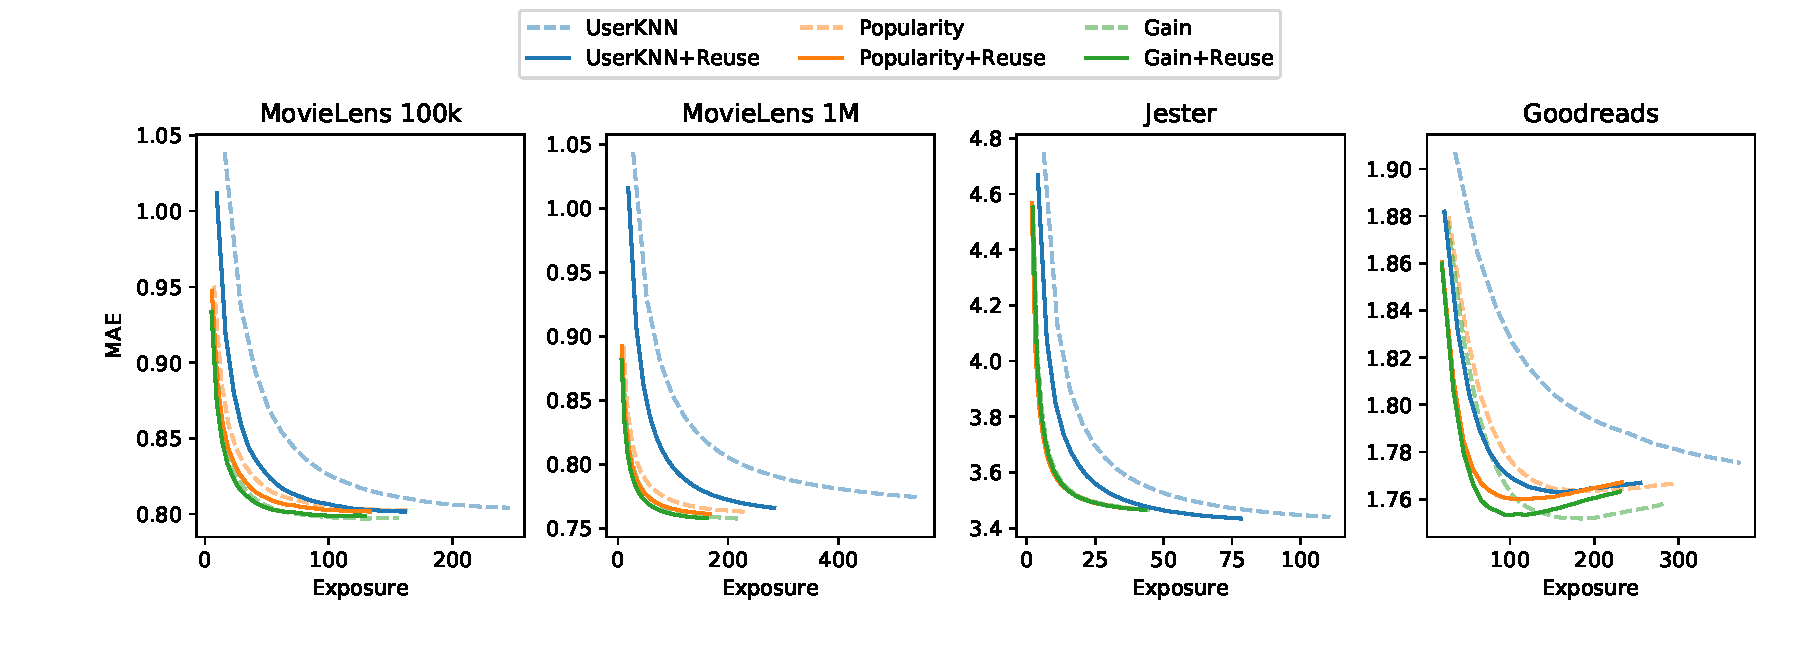
\includegraphics[width=\linewidth]{figures/tradeoff.pdf}
    \caption{The relationship between MAE and Exposure illustrating the accuracy-privacy trade-off for the baseline \emph{UserKNN} and our neighborhood reuse methods utilized in \emph{ReuseKNN}. As can be seen, our methods exhibit less Exposure for less increase of MAE compared to traditional \emph{UserKNN} and as such, improve users' accuracy-privacy trade-offs. In general, the explicit and personalized \emph{Gain+Reuse} method yields the best results. However, \emph{UserKNN+Reuse} for \emph{Jester} and \emph{Gain} for \emph{Goodreads} yield marginally better $\mathrm{MAE}$ than \emph{Gain+Reuse} but substantially increase $\mathrm{Exposure}$. Furthermore, we highlight that for \emph{MovieLens 1M}, \emph{Gain+Reuse} keeps \emph{UserKNN}'s level of accuracy, but only for less than 10\% of its Exposure.
    }
    \label{fig:results_trade-off}
\end{figure}

As we can see, traditional \emph{UserKNN} yields the worst accuracy-privacy trade-off for all four datasets.
Naively extending traditional \emph{UserKNN} with explicit neighborhood reuse, i.e., \emph{UserKNN+Reuse}, results in a substantial improvement.
For all of our remaining neighborhood reuse methods, it is possible to decrease the Exposure whilst preserving a low MAE.
Furthermore, it is important to note that explicit neighborhood reuse methods always lead to a better accuracy-privacy trade-off than its implicit counterpart.
This supports our intuition that reusing neighbors corresponds to decreased exposure of users.
Moreover, among our neighborhood reuse methods, the personalized and implicit \emph{Gain} method and the personalized and explicit \emph{Gain+Reuse} method perform best.
This observation indicates that personalized neighborhood reuse methods are beneficial in terms of decreasing users' exposure whilst keeping accurate recommendations.
For the \emph{Jester} dataset, \emph{Popularity}, \emph{Popularity+Reuse}, \emph{Gain}, and \emph{Gain+Reuse} perform equally well.
Thus, for \emph{Jester}, there is no advantage of using explicit neighborhood reuse methods over implicit neighborhood reuse methods, plus, personalized neighborhood reuse methods are not beneficial over unpersonalized neighborhood reuse methods.
Due to this dataset comprising only 100 items, we hypothesize that personalization cannot improve recommendations substantially, since all users rated a similar set of items.
In the same vein, also explicit neighborhood reuse methods are not able to yield any further improvement, as the average user already rated 60\% of items. 
That means that the implicit neighborhood reuse methods provide a neighborhood that already rated most items a user could query recommendations for.
Thus, we conclude that for a dataset with a very limited number of items, e.g., \emph{Jester}, personalized and explicit neighborhood reuse methods are not beneficial over unpersonalized and implicit neighborhood reuse methods.

\begin{figure}[!t]
    \centering
    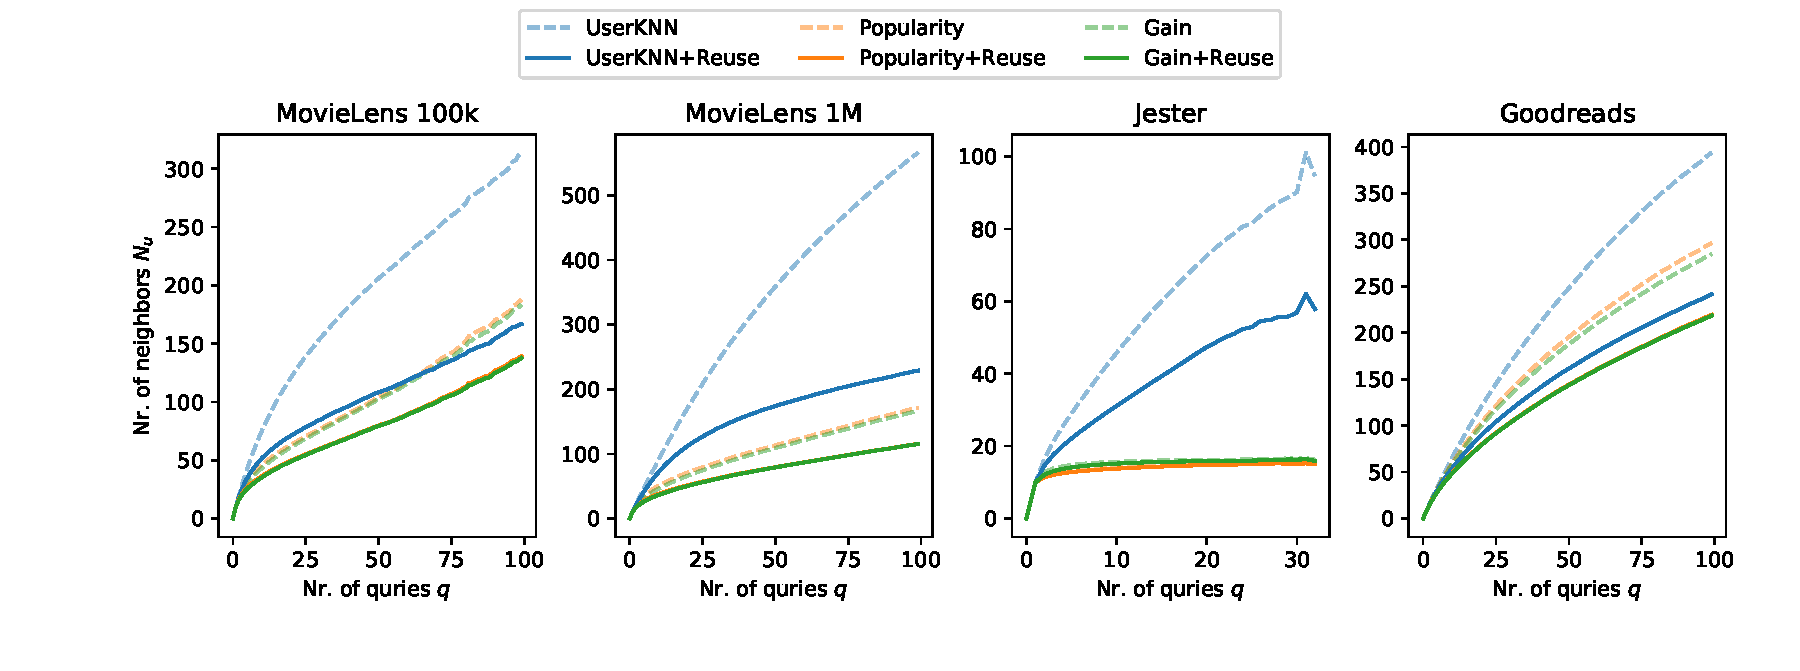
\includegraphics[width=\linewidth]{figures/neighborhood.pdf}
    \caption{The average number of neighbors per user after querying $q$ recommendations. Here, for \emph{MovieLens 100k}, \emph{MovieLens 1M}, and \emph{Goodreads}, we only visualize the average $\mathrm{Neighbors}@q$ for $q \leq 100$.
    \emph{Jester} comprises only 30 queries due to its small set of items. 
    Furthermore, we utilize $k=10$ neighbors to generate recommendations for this experiment. 
    We note that the average $\mathrm{Neighbors}@q$ increases more strongly for \emph{UserKNN} than for our implicit and explicit neighborhood reuse methods utilized in our \emph{ReuseKNN} recommender system. Furthermore, the explicit and personalized \emph{Gain+Reuse} and the explicit and unpersonalized \emph{Popularity+Reuse} methods perform best with respect to limiting the growth of users' neighborhood.}
    \label{fig:results_neighborhood}
\end{figure}

\subsection{Neighborhood Growth}
To increase privacy of users, our novel \emph{ReuseKNN} recommender system utilizes neighborhood reuse methods to reduce the neighborhood $N_u$ of a target user $u$.
As such, users are required to participate in the generation of recommendations for less target users and thus, their exposure is reduced, which leads to increased privacy.
Figure~\ref{fig:results_neighborhood} illustrates the average size of users' neighborhood after querying $q$ recommendations. 
For all of our four datasets, traditional \emph{UserKNN} performs worst.
That means that the number of a user's neighbors strongly increases for \emph{UserKNN}, which is not the case for our neighborhood reuse methods.
Especially after the first few recommendation queries, our neighborhood reuse methods yield substantially smaller neighborhoods than \emph{UserKNN}.
In general, it is noteworthy that \emph{Popularity} and \emph{Gain} reuse neighbors to the same degree, which means that they equally increase users' privacy.
In our previous results regarding the accuracy-privacy trade-off in Figure~\ref{fig:results_trade-off}, we observed that \emph{Gain} yields a better trade-off than \emph{Popularity}.
Since both methods equally increase privacy, this means that our personalized \emph{Gain} approach is able to persist higher accuracy than our unpersonalized \emph{Popularity} approach.
This also means that \emph{Gain+Reuse} is advantageous over \emph{Popularity+Reuse}.

Since our neighborhood reuse methods outperform traditional \emph{UserKNN} only after the first few recommendation queries, we suspect that they utilize the first few recommendation queries to build a sufficiently reusable neighborhood.
After this phase, our neighborhood reuse methods exploit this well-formed neighborhood of a target user $u$ and minimize the growth of $u$'s neighborhood $N_u$.
This effect is most prominent for \emph{Jester}.
Here, \emph{UserKNN} increases the average number of a user's neighbors constantly even after multiple recommendation queries.
For our neighborhood reuse methods, the average size of the neighborhood only increases marginally after the first few recommendation queries. 
Hence, most succeeding recommendations are generated based on reused neighbors in our novel \emph{ReuseKNN} recommender system.

\begin{figure}[!t]
    \centering
    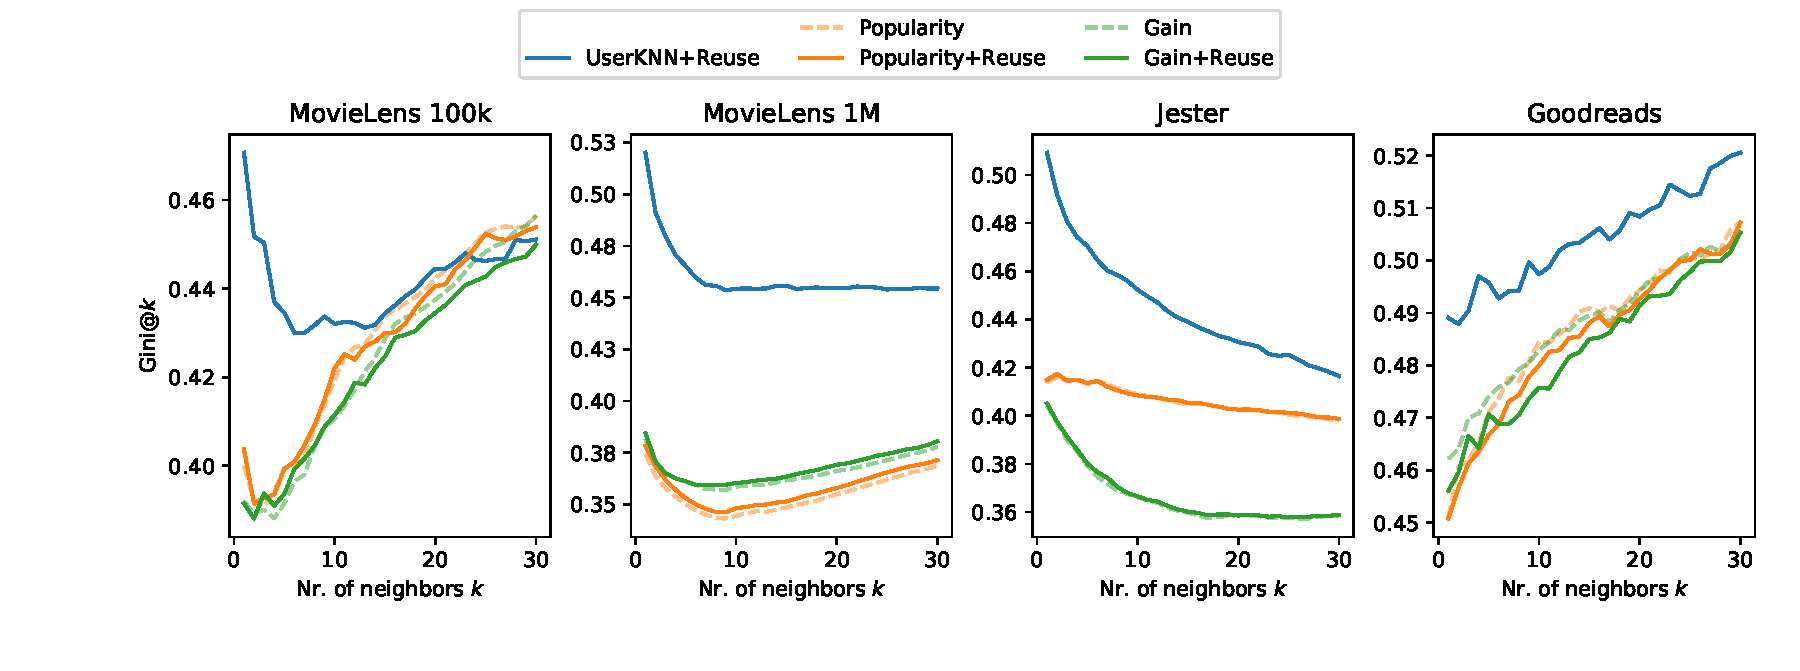
\includegraphics[width=\linewidth]{figures/gini.pdf}
    \caption{The number of neighbors used for generating recommendations plotted over the degree to which our neighborhood reuse methods show a neighborhood bias, as measured by the Gini-index of the $\Delta \text{TradeOff}@k$ distribution. 
    It can be seen that naively reusing neighbors in traditional \emph{UserKNN}, i.e., \emph{UserKNN+Reuse}, yields to a severe bias towards some neighbors.
    In contrast, our neighborhood reuse methods tend to preserve users' accuracy-privacy trade-offs. In the case of \emph{Jester}, we observe that the neighborhood bias diminishes when the number of neighbors increases. Thus, target users' tend to have different neighborhoods.
    }
    \label{fig:results_gini}
\end{figure}

\subsection{Neighborhood Bias}
Our proposed \emph{ReuseKNN} recommender system utilizes a small set of reused neighbors, which is different to the neighborhood utilized by \emph{UserKNN}.
In particular, we outlined in Section~\ref{subsubsec:acc_priv_bias} that for a single target user, \emph{ReuseKNN} influences accuracy of target users' recommendations and privacy of neighbors.
To test whether \emph{ReuseKNN} tends to reuse the same neighborhood for all target users, i.e., neighborhood bias, we proposed our $\mathrm{Gini}@k_\nu$ measurement.
%Furthermore, we proposed our $\mathrm{Gini}@k_\nu$ measurement that quantifies to what extent the distribution of the users' accuracy-privacy trade-offs generated by neighborhood reuse method $\nu$'s is different from the distribution generated by traditional \emph{UserKNN}.
The closer $\mathrm{Gini}@k_\nu$ is to 0, the better $\nu$ preserves the accuracy-privacy trade-off distribution of \emph{UserKNN} and the less biased $\nu$ is towards the same set of neighbors.
%More detailed, the distribution of users' accuracy-privacy trade-offs generated by \emph{ReuseKNN} with neighborhood reuse method $\nu$ is not biased towards a small set of neighbors.

In Figure~\ref{fig:results_gini}, we relate $\mathrm{Gini}@k$ to the number of neighbors $k$ used for generating recommendations.
It can be observed that naively reusing neighbors in traditional \emph{UserKNN}, i.e., \emph{UserKNN+Reuse}, leads to the strongest bias, i.e., high $\mathrm{Gini}@k$ values.
In contrast, \emph{Popularity}, \emph{Popularity+Reuse}, \emph{Gain}, and \emph{Gain+Reuse} are less biased, i.e., low $\mathrm{Gini}@k$ values.
Interestingly, for \emph{Jester}, the bias decreases, if more neighbors are used for generating recommendations.
For all remaining datasets, i.e., \emph{MovieLens 100k}, \emph{MovieLens 1M}, and \emph{Goodreads}, the opposite is true.
The strong bias indicates that \emph{ReuseKNN} is biased towards some neighbors, i.e., the accuracy-privacy trade-off distribution is different to \emph{UserKNN}.
We suspect that the larger $k$, the higher the probability that some reusable users are neighbors of most target users.
This leads to those neighbors being increasingly exposed to lots of target users and thus, leading to a severe bias towards them. 
The absence of this effect for \emph{Jester} could be explained by the low number of items within this dataset. 
In detail, we hypothesize that due to users providing ratings for on average 60\% of items, a target user $u$ could reuse its neighbors and does not need to add new neighbors.
It makes sense that $\mathrm{Exposure@k(n)}$ of users does not change, if their neighborhoods do not change.
Therefore, the low number of items in the \emph{Jester} dataset leads to not adding new neighbors to users' neighborhoods, which means that the distribution of accuracy-privacy trade-offs remains similar to the one of traditional \emph{UserKNN}.


\section{Related Work}
With increasing popularity of real-world recommender systems, research discovered a multitude of severe privacy issues.
In particular, \cite{shyong2006you} listed three privacy-related problems in collaborative filtering: (i) Exposing users' data, (ii) Maliciously influencing what is recommended, and (iii) Sabotaging the recommender system to generate low-accuracy recommendations.
In our work at hand, we focus on the issue of exposing a user's rating data to other users, without consent of the affected users, i.e., data breaches, in user-based \emph{KNN} recommender systems. Additionally, we review related research in the area of privacy-aware recommender systems.

%Furthermore, privacy-aware recommender systems have been developed, to increase users' privacy.
%Here, the majority of state-of-the-art research utilizes concepts like \emph{Homomorphic Encryption}~\cite{gentry2009fully}, \emph{Differential Privacy}~\cite{dwork2014algorithmic}, or \emph{Federated Learning}~\cite{konevcny2015federated,mcmahan2017communication}.

\vspace{2mm} \noindent \emph{Data breaches in recommender systems.}
\cite{ramakrishnan2001being} pinpoint the generation of recommendations by a target user's neighbors as severe threat to its neighbors' privacy.
Serendipitous recommendations yield a unique connection between target user and its neighbors.
This unique connection moreover, could uncover neighbors' rating data, or even reveal the identity of them within the recommendation database.
Furthermore, the authors find that through probing, i.e., adding specific ratings and querying recommendations, a target user could actively increase the risk of compromising its neighbors' privacy.
Among other attacks,  \cite{calandrino2011you} propose so called \emph{Sybil}-attacks in user-based \emph{KNN} recommender systems, in which limited knowledge of a victim's data is utilized to construct $k$ fake users, i.e., \emph{Sybils}, with high similarity to the victim.
In detail, the $k$-th \emph{Sybil} queries a recommendation and thus, its neighborhood likely comprises the $k-1$ remaining \emph{Sybils} and the victim.
By observing the recommendation through the $k$-th \emph{Sybil}, an attacker could easily cancel out the contribution of the $k-1$ \emph{Sybils} and reveal the rating data of the victim.
However, \cite{frey2015collaborative} show that this attack's effectiveness strongly depends on the amount of knowledge of the victim's data.
This knowledge by itself already poses a breach of the victim's privacy.
Moreover, the victim's data could also be utilized to infer sensitive and private attributes.
For example, \cite{weinsberg2012blurme} trained a classifier on data from a small set of users, who provided their gender.
Then, they demonstrate that by applying their classifier on other users' rating data, one could easily infer the gender of 80\% of these users.


\vspace{2mm} \noindent \emph{Privacy-aware recommender systems.}
\cite{badsha2017privacy} encrypt users' data with a \emph{Homomorphic Encryption}~\cite{gentry2009fully} scheme.
Specifically, the recommender system generates recommendations based on the encrypted data, which is subsequently decrypted by the target user.
As such, users' data is not exposed to the recommender system, or to other users.
\emph{Homomorphic Encryption}'s strong privacy guarantees also leads to its suitability within sensitive domains, e.g., medical data~\cite{zhang2021privacy}.
However, one problem of \emph{Homomorphic Encryption} is its poor efficiency.
To alleviate this issue, \cite{tang2016privacy,kikuchi2012accuracy} utilize a variant with lower privacy guarantees, but improved efficiency.
Parallel to \emph{Homomorphic Encryption}, also \emph{Differential Privacy}~\cite{dwork2014algorithmic} and obfuscation have been used to develop privacy-aware recommender systems.
In general, random noise is added to users' rating data to hide its real value.
However, \cite{berkovsky2012impact} demonstrate that data obfuscation seriously impacts the accuracy of recommendations.
Therefore, the level of random noise has to be fine-tuned to ensure privacy whilst not compromising the accuracy of recommendations~\cite{mcsherry2009differentially}.
In the same vein, \cite{meng2018personalized} utilize different noise levels depending on the sensitivity of data.
On sensitive data, noise and thus, privacy, shall be increased, whereas for non-sensitive data, a lower level of noise is sufficient.
Additionally, in \emph{Matrix Factorization} for example, noise could not only be added to users' data, but also to the gradient and the recommender system's output~\cite{berlioz2015applying}.
Research also utilized \emph{Differential Privacy} to construct privacy-aware user-based \emph{KNN} recommender systems~\cite{lu2015security,zhu2014effective}.
However, \cite{okkalioglu2016reconstructing} show that obfuscated data could be reconstructed, if the obfuscation is performed inconsistently.
%In contrast, multiple privacy-aware recommender systems do not obfuscate the data to protect users' privacy, but instead, rely on modifications to their architecture.
%In detail, \cite{wang2015decentralized} and~\cite{kermarrec2010application} present decentralized recommender systems, in which data and computation are distributed among users.
%As such, no central server is needed and thus, privacy is increased due to the absence of a single point of data breach.
%\cite{duriakova2019pdmfrec} go one step further and propose a \emph{Decentralized Matrix Factorization} framework, in which only non-sensitive information are shared among a user's neighbors.
%Specifically, only the updates to the item-factors are shared and thus, the more sensitive user-factors are protected.
Recent research does not obfuscate data but takes another approach by utilizing \emph{Federated Learning}~\cite{ammad2019federated,chen2018federated}.
Here, users do not share their data with the recommender system, but share only their updates to the model.
This way, no data ever leaves the user's device and as such, it is protected against breach.
However, we note that \emph{Federated Learning} is prone to a multitude of attacks that could compromise a user's privacy~\cite{nasr2019comprehensive}.
Therefore, recent research works~\cite{anelli2021put,robustnessofmetamf} propose to allow users to reduce the amount of data they share with the recommender system.
Additionally, both works provide evidence that only a small fraction of a user's data is needed to provide highly-accurate recommendations.

These works aimed to increase a user's privacy by reducing its data.
In our work, we go into a similar direction, but instead of addressing the accuracy-privacy trade-off by reducing a user's data, we aim to address this trade-off by reducing a user's exposure to other users.



\section{Conclusion \& Future Work}
This study presents the privacy-benefit of reusing neighbors in user-based \emph{KNN} recommender systems.
We outlined our novel \emph{ReuseKNN} recommender system and leveraged a trade-off between similarity and reusability as proxy to users' accuracy-privacy trade-offs.
Moreover, we demonstrated \emph{ReuseKNN} on four diverse datasets from different domains and illustrated its superiority in terms of users' accuracy-privacy trade-off to traditional \emph{UserKNN}.
In detail, by rendering a neighbor's reusability dependent of the target user, we found that \emph{ReuseKNN} substantially improves users' privacy at no or only marginal cost of accuracy.
Furthermore, experiments showed that the growth of a user's neighborhood is far more limited than in traditional \emph{UserKNN}.
Plus, we provided strong evidence that even though a single target user's recommendations rely on a small neighborhood, \emph{ReuseKNN} does not bias recommendations for many target users on the same set of neighbors.
Instead, we concluded that \emph{ReuseKNN} generates distinct neighborhoods for each individual target user.
Our \emph{ReuseKNN} recommender system exploits reusage of neighbors to increase users' privacy.
With that we desire to give an example of how simple modifications of the inner workings of traditional recommendation algorithms could alleviate their users' privacy issues.

In our future research, we strive to not only measure recommendation quality by accuracy, but also consider more sophisticated quality measurements as, e.g., serendipity and diversity.
%Additionally, we aim to improve our \emph{ReuseKNN} recommender system further, by designing artificial users that exhibit maximal reusability, in addition to providing accurate recommendations. \dk{this needs more details, I think the reader does not understand what is meant with artificial user and with maximum reusability + here you could also include the point about securing high-exposed users such as Bob}
Moreover, we aim to protect high-exposed users, i.e., reused neighbors such as \emph{Bob}, by constructing fake neighbors that are reused instead of real users.
For example, a fake neighbor's rating data could comprise parts of \emph{Bob}'s ratings in addition to fake ratings.
As such, we plan to preserve accuracy of recommendations, whilst increasing the reusability of the fake neighbor and thus, protect rating data of real users.

%\pmu{Shortcomings of Gain: Measures the fraction of a student's rated items in the trainset, a mentor covers ($|I^{mentor}_{train} \cap I^{student}_{train}| / |I^{student}_{train}|$). We choose the mentor that has the highest coverage of a student. The problem occurs, if the mentor rated exactly the same items as the student ($I^{mentor}_{train} = I^{student}_{train}$). Then, the gain is maximal at 1, but we cannot use this mentor in the future, since the student already used all of the mentor's data in the training phase.}

%\section{Acknowledgements}
%\dk{only needed for cr-version}
%\pmu{This work is supported by the H2020 project TRUSTS (GA:871481)} and the ``DDAI'' COMET Module within the COMET – Competence Centers for Excellent Technologies Programme, funded by the Austrian Federal Ministry (BMK and BMDW), the Austrian Research Promotion Agency (FFG), the province of Styria (SFG) and partners from industry and academia. The COMET Programme is managed by FFG.

% TRUSTS acknowledgements
%The research leading to these results has received funding from the European Union’s Horizon 2020 Research and Innovation Programme, under Grant Agreement no 871481 – Trusted Secure Data Sharing Space (TRUSTS), from the H2020-ICT-2018-20/H2020-ICT-2019-2 Call.

%%
%% The acknowledgments section is defined using the "acks" environment
%% (and NOT an unnumbered section). This ensures the proper
%% identification of the section in the article metadata, and the
%% consistent spelling of the heading.


%%
%% The next two lines define the bibliography style to be used, and
%% the bibliography file.
\bibliographystyle{ACM-Reference-Format}
\bibliography{references}

%%
%% If your work has an appendix, this is the place to put it.


\end{document}
\endinput
%%
%% End of file `sample-acmtog.tex'.
